\section{Eddie final setup and bringup}
%=========================================================================================================================
%-------------- 1.1 GETTING TO KNOW EDDIE
%=========================================================================================================================
\subsection{Getting to know Eddie}
Eddie is a versatile mobile robotics development platform. Eddie is equipped with 3D vision capabilities, utilizing the Microsoft Kinect, allowing it to perceive its surroundings in three dimensions. The platform is versatile, supporting applications like autonomous navigation, machine vision system development, tele-presence robots, personal assistant robots, security and surveillance robots, and crowd interaction and advertising. \\
\newline
%-------------------------------------------------------------------------------------------------------------------------
%....................1.1.1 HARDWARE SUBSYSTEMS 
%-------------------------------------------------------------------------------------------------------------------------
\subsubsection{Hardware Subsystems}
Eddie is a differential drive robot featuring a microcontroller with an integrated PID, two optical wheel encoders, two PWM driven motors, and two lead-acid batteries. 
The robot's structure comprises a pair of top and bottom decks, along with an undercarriage designed to hold the batteries securely.\\
\begin{figure}[H]
	\centering
	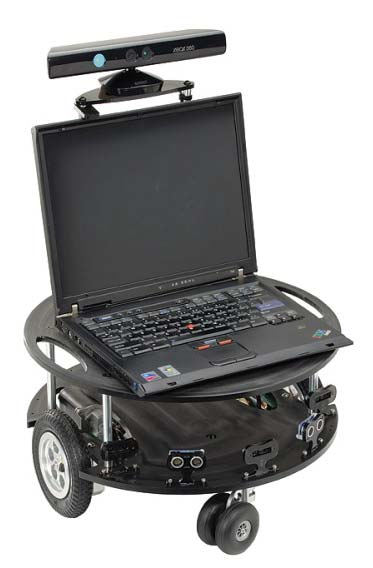
\includegraphics[width=0.8\linewidth]{figures/platform.png}
	\caption{Eddie Platform}
	\label{fig:platform}
\end{figure}

\textbf{Range Sensors.} On its base, there are five distance sensors placed for collision avoidance. This sensor array comprises three infrared (IR) sensors and two ultrasonic sensors.\\

\textbf{Wheel Encoders.} The 36-position Quadrature Encoders offer a reliable method to track the position and speed of each wheel continuously. When used with the included Encoder disks, each Encoder assembly provides a basic resolution of 36 positions per rotation. However, since there are two sensors in each assembly, the potential resolution increases to 144 positions per full tire rotation. This equates to a linear resolution of approximately 0.13 inches of travel per drive assembly when using the standard six-inch tires. It's important to note that the actual resolution may be limited by the amount of backlash in the gear motor assemblies, which is approximately +/- 0.175 linear inches.
The Position Controllers are compatible with any microcontroller via a single-wire half-duplex asynchronous serial communication (UART) bus.\\

\textbf{Board.} The Eddie Control Board provides a complete single-board solution to control the Eddie Robot Platform. It utilizes the powerful Propeller P8X32A microcontroller, boasting eight 32-bit cores for impressive performance and versatility. The board incorporates high-current motor drivers, an eight-channel 10-bit ADC, and ample digital I/O options. It communicates via a USB mini-B connector, which enumerates as a serial COM port.\\
\begin{figure}[H]
	\centering
	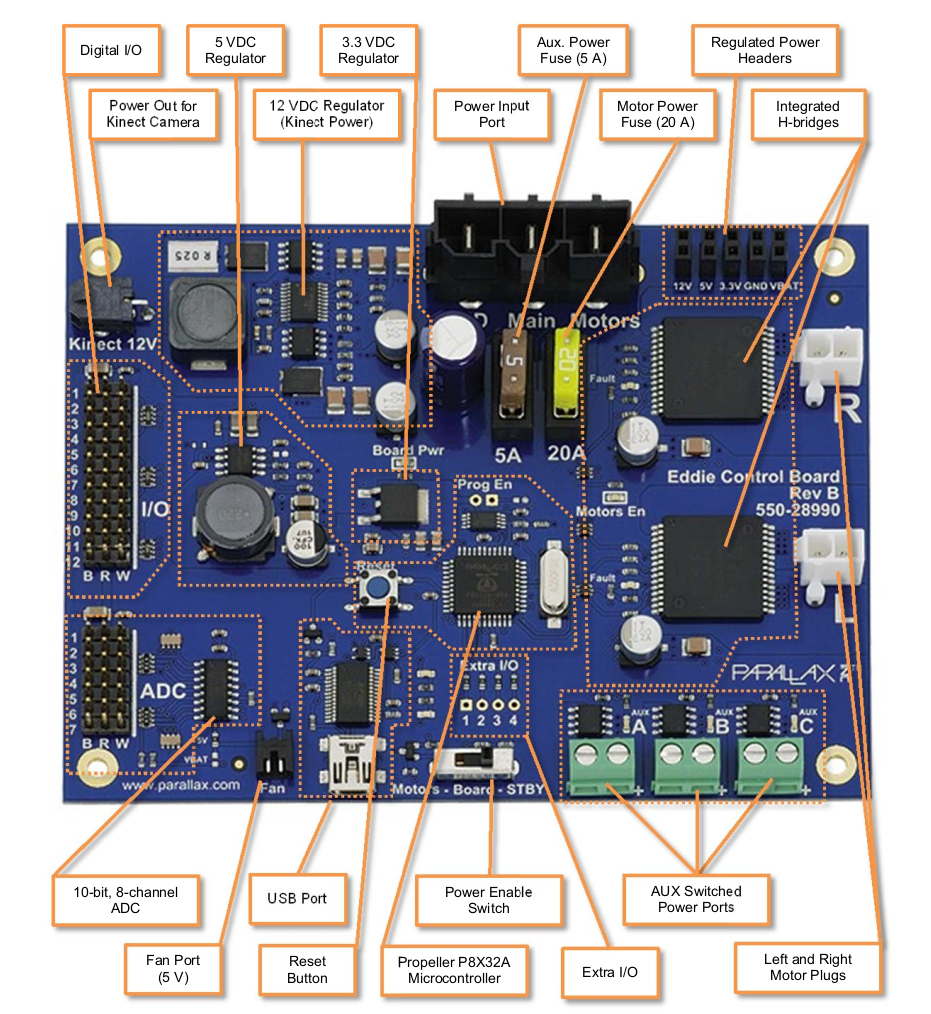
\includegraphics[width=0.8\linewidth]{figures/board-overview.png}
	\caption{Board Overview}
	\label{fig:boardOverview}
\end{figure}
Most of the Propeller’s 32 general purpose I/O pins are used to interface with on-board peripherals, or connect to headers for sensor interfacing. The Digital I/O pins are brought out to twelve 3-pin headers near the edge of the board. The order of the pins from left to right is: Ground, 5V, Signal. 
\begin{itemize}
    \item The 1st and 2nd pins are connected to our two ultrasonic sensors.
\end{itemize}
    
For the analog to digital converter, the board is equipped with the Microchip MCP3008 which is an 8-channel, 10-bit ADC.
\begin{itemize}
    \item The left-most IR Sensor cable is connected to “AD1”, the center IR sensor to “AD2”, and the right-most IR Sensor to “AD3”.
\end{itemize}

The three-pin cable from the right Position Controller is connected to Pin-set 11 in the “Encoders” section of the Control Board.\\

\textbf{Camera.} The Kinect for Xbox 360 is a combination of software and hardware, featuring a range chipset technology by PrimeSense, which uses an infrared projector and camera to determine the location of nearby objects in 3D. 

The Kinect sensor consists of an RGB camera, depth sensor, and microphone array, allowing for full-body 3D motion capture, facial recognition, and voice recognition capabilities. The depth sensor employs an infrared laser projector and monochrome CMOS sensor to capture 3D video data under any lighting conditions, with an adjustable sensing range and automatic calibration for different environments.\\

The software technology of Kinect enables advanced gesture recognition, facial recognition, and voice recognition, making it capable of simultaneously tracking up to six people. The Kinect's various sensors output video at frame rates ranging from approximately 9 Hz to 30 Hz, with different resolutions and color formats. The sensor has a practical ranging limit of 1.2–3.5 meters and a field of view of 57° horizontally and 43° vertically, providing a high resolution of over 1.3 mm per pixel. To power the motorized tilt mechanism of the Kinect sensor, a proprietary connector combining USB communication and additional power is used, while older models require a special power supply cable that splits the connection into separate USB and power connections.
\begin{figure}[H]
	\centering
	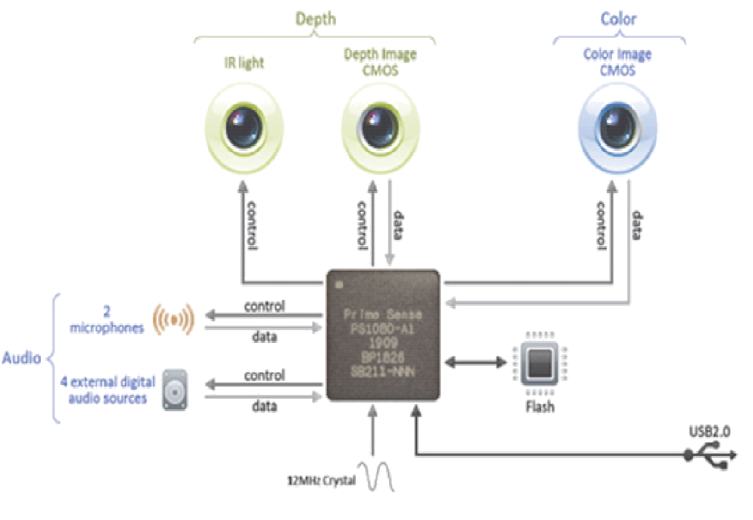
\includegraphics[width=0.8\linewidth]{figures/kinect-components.png}
	\caption{Kinect Components}
	\label{fig:kinectComponents}
\end{figure}
%-------------------------------------------------------------------------------------------------------------------------
%....................1.1.2 CONTROL BOARD FIRMWARE COMMAND SET 
%-------------------------------------------------------------------------------------------------------------------------
\subsubsection{Control Board Firmware Command Set}
The Eddie Control Board is a complete robot controller and sensor-interface solution. Parallax’s ready-to-go Eddie Control Board firmware, designed for the Eddie Robot Platform provides an easy-to-use serial command interface to control and manage all of the on-board peripheral electronics such as motor drivers, digital I/O, and analog to digital converter (ADC) channels.

The Eddie Control Board communicates over USB; and when connected to a PC, the board enumerates as a serial COM port. Configure the COM port to use these settings of 115.2 kBaud, 8-bit character size, 1 stop bit and no parity.

All commands adhere to the same general format which is shown below:\\
Input: \: \, \, \qquad \qquad \qquad \textcolor{OliveGreen}{<cmd>}[\textcolor{BrickRed}{<WS>}\textcolor{OliveGreen}{<param1>}...\textcolor{BrickRed}{<WS>}\textcolor{OliveGreen}{<paramN>}]\textcolor{BrickRed}{<CR>}\\
Response (Success):\qquad [\textcolor{OliveGreen}{<param1>}...\textcolor{BrickRed}{<WS>}\textcolor{OliveGreen}{<paramN>}]\textcolor{BrickRed}{<CR>}\\
Response (Failure): \qquad \textcolor{RoyalBlue}{ERROR}[\textcolor{BrickRed}{<SP>}-\textcolor{BrickRed}{<SP>}\textcolor{OliveGreen}{<verbose\_reason>}]\textcolor{BrickRed}{<CR>}\\

In this format:
\begin{itemize}
    \item \textcolor{OliveGreen}{<cmd>} represents the command mnemonic.
    \item \textcolor{OliveGreen}{<param1>}...\textcolor{OliveGreen}{<paramN>} are optional parameters required by the command or mode. Numbers are always entered as hexadecimal values, and signed values use two's complement.
    \item \textcolor{BrickRed}{<WS>} refers to one or more whitespace characters, which can be spaces (ASCII 32) or tabs (ASCII 9).
    \item \textcolor{BrickRed}{<CR>} is a single carriage-return character (ASCII 13).
    \item \textcolor{BrickRed}{<SP>} is a single space character (ASCII 32).
    \item \textcolor{OliveGreen}{<verbose\_reason>} is an optional error message displayed when verbose mode is enabled (using the VERB command).
\end{itemize}

Allowed characters are in the ASCII range from 32 to 126, except for carriage return (ASCII 13) and tab (ASCII 9).
Commands can have up to 254 characters, including the terminating carriage return character. Anything beyond this limit is ignored as an invalid command. The command handler only processes and responds after receiving the carriage return character.

\begin{table}[H]
\caption{Eddie Command Set Description: \textit{Interface}}
\label{tab:eddie_commands}
\begin{tabular}{|p{4em}|p{6em}|p{6em}|p{9em}|p{11em}|}
\hline
\textbf{\large Cmd} & \textbf{\large Input Params} & \textbf{\large Return Params} & \textbf{\large Values} & \textbf{\large Description} \\ \hline \hline
HWVER &  & \textit{\textbf{<version>}} & \textit{\textbf{version}}=0..FFFF & Get hardware version \\ \hline
VER &  & \textit{\textbf{<version>}} & \textit{\textbf{version}}=0..FFFF & Get firmware version \\ \hline
VERB & \textit{\textbf{<mode>}} &  & \textit{\textbf{mode}}= 0(off), 1(on) & Set verbose mode \\ \hline
WATCH & \textit{\textbf{<mode>}} &  & \textit{\textbf{mode}}= 0(off), 1(on) & Set watch mode \\ \hline
BLINK & \textit{\textbf{<pin>}}\textit{\textbf{<rate>}} &  & \textit{\textbf{pin}}=0.. 1F\newline\textit{\textbf{rate}}=0..FFFF & Toggle pin at a specified rate in increments of 0.1Hz \\ \hline
\end{tabular}
\end{table}

\begin{table}[H]
\caption{Eddie Command Set Description: \textit{I/O Control}}
\label{tab:eddie_commands}
\begin{tabular}{|p{3em}|p{4.5em}|p{4.5em}|p{7.5em}|p{14em}|}
\hline
\textbf{\large Cmd} & \textbf{\large Input Params} & \textbf{\large Return Params} & \textbf{\large Values} & \textbf{\large Description} \\ \hline \hline
IN & \textit{\textbf{<bitmask>}} &  & \textit{\textbf{bitmask}}=0..7FFFF & Set GPIO pins in bitmask to inputs \\ \hline
OUT & \textit{\textbf{<bitmask>}} &  & \textit{\textbf{bitmask}}=0..7FFFF & Set GPIO pins in bitmask to outputs \\ \hline
LOW & \textit{\textbf{<bitmask>}} &  & \textit{\textbf{bitmask}}=0..7FFFF & Set GPIO pins in bitmask to low (only applies to output pins) \\ \hline
HIGH & \textit{\textbf{<bitmask>}} &  & \textit{\textbf{bitmask}}=0..7FFFF & Set GPIO pins in bitmask to high (only applies to output pins) \\ \hline
INS & & \textit{\textbf{<bitmask>}} & \textit{\textbf{bitmask}}=0..7FFFF & Get GPIO pins currently set as inputs \\ \hline
OUTS & & \textit{\textbf{<bitmask>}} & \textit{\textbf{bitmask}}=0..7FFFF & Get GPIO pins currently set as outputs \\ \hline
LOWS & & \textit{\textbf{<bitmask>}} & \textit{\textbf{bitmask}}=0..7FFFF & Get GPIO pins currently set as low \\ \hline
HIGHS & & \textit{\textbf{<bitmask>}} & \textit{\textbf{bitmask}}=0..7FFFF & Get GPIO pins currently set as high \\ \hline
READ & & \textit{\textbf{<bitmask>}} & \textit{\textbf{bitmask}}=0..7FFFF & Get current state (high/low) of all GPIO pins \\ \hline
\end{tabular}
\end{table}

\begin{table}[H]
\caption{Eddie Command Set Description: \textit{Sensor Interfacing}}
\label{tab:eddie_commands}
\begin{tabular}{|p{3em}|p{4.5em}|p{8.5em}|p{7.5em}|p{14em}|}
\hline
\textbf{\large Cmd} & \textbf{\large Input Params} & \textbf{\large Return Params} & \textbf{\large Values} & \textbf{\large Description} \\ \hline \hline
SPNG & \textit{\textbf{<bitmask>}} &  & \textit{\textbf{bitmask}}=0..FFFF & Set pins in bitmask to act as GPIO pins \\ \hline
SGP & \textit{\textbf{<bitmask>}} &  & \textit{\textbf{bitmask}}=0..7FFFF & Set pins in bitmask to act as GPIO pins \\ \hline
PING & & \textit{\textbf{<value1>}}[\textit{\textbf{<value2>}}\newline...\textit{\textbf{<valueN>}}] & \textit{\textbf{value}}=0,12..B54 & Get PING))) sensor sonar measurements (one 12-bit value per sensor) \\ \hline
ADC &  & \textit{\textbf{<value1>}}...\textit{\textbf{<value8>}} & \textit{\textbf{value}}=0..FFF & Get all ADC values (12-bit values) \\ \hline
\end{tabular}
\end{table}

\begin{table}[H]
\caption{Eddie Command Set Description: \textit{Motor Control}}
\label{tab:eddie_commands}
\begin{tabular}{|p{3em}|p{6.7em}|p{5.7em}|p{8.5em}|p{15em}|}
\hline
\textbf{\large Cmd} & \textbf{\large Input Params} & \textbf{\large Return Params} & \textbf{\large Values} & \textbf{\large Description} \\ \hline \hline
GO & \textit{\textbf{<left>}}\textit{\textbf{<right>}} &  & \textit{\textbf{left/right}}=80..7F & Set motor power (signed byte) \\ \hline
GOSPD & \textit{\textbf{<left>}}\textit{\textbf{<right>}} &  & \textit{\textbf{left/right}}=8000..7FFF & Set motor speed (signed word) \\ \hline
STOP & \textit{\textbf{<dist>}} &  & \textit{\textbf{dist}}=0..FFFF & Slow to a stop over specified distance \\ \hline
TRVL & \textit{\textbf{<dist>}}\textit{\textbf{<speed>}} &  & \textit{\textbf{dist}}=8000..7FFF \newline \textit{\textbf{speed}}=1..7F or 1..FF & Travel a specified distance in a straight line, ramping up to a maximum specified speed \\ \hline
TURN & \textit{\textbf{<angle>}}\textit{\textbf{<speed>}} &  & \textit{\textbf{dist}}=8000..7FFF \newline \textit{\textbf{speed}}=1..7F or 1..FF & Rotate in place by a specified angle, ramping up to a maximum specified speed \\ \hline
STOP & \textit{\textbf{<rate>}} &  & \textit{\textbf{rate}}=1..7F or 1..FF & Set rate of acceleration/deceleration \\ \hline
SPD & & \textit{\textbf{<left>}}\textit{\textbf{<right>}} & \textit{\textbf{left/right}}=8000..7FFF & Get the current average speed (positions per
second) for both wheels \\ \hline
HEAD & & \textit{\textbf{<angle>}} & \textit{\textbf{angle}}=0..168 \newline(decimal 0..359) & Get the current heading (in degrees) relative to
start \\ \hline
DIST & & \textit{\textbf{<left>}}\textit{\textbf{<right>}} & \textit{\textbf{left/right}}=80000000..\newline 7FFFFFFF & Get the current average speed (positions per second) for both wheels \\ \hline
RST &  &  &  & Reset the distance and heading values to 0 \\ \hline
\end{tabular}
\end{table}
%-------------------------------------------------------------------------------------------------------------------------
%....................1.1.3 SOFTWARE SUBSYSTEMS
%-------------------------------------------------------------------------------------------------------------------------
\subsubsection{Software Subsystems}
\textbf{Robot Communication: \textcolor{Plum}{\texttt{\Large eddiebot\_bringup}}}\\
The communication with the board involves establishing a connection between the robot control board and our ROS2 programs, enabling seamless data exchange. This software acts as a  pathway that conveys and receives data between two of our major hardware components. Specifically, this sub-system serves as the means to convey the desired velocity information from the control system to be executed by the robot's firmware board. \\

\textbf{Description: \textcolor{Plum}{\texttt{\Large eddiebot\_description}}}\\
This package contains files and data used to describe the structure of eddie. It includes URDF files to define the physical properties and kinematic structure of eddie. This package enables accurate simulation of Eddie's structure and movement within the ROS environment. This is crucial for visualizing and controlling the robot in a virtual space before deploying it in the physical world.

The \texttt{diff\_drive} plugin is a component added to the URDF files to simulate the differential drive mechanism that eddie uses.

The \texttt{joint\_state\_publisher} plugin is another component added to the URDF files. It is used to simulate the movement of Eddie's wheels. \texttt{joint\_state\_publisher} helps in updating the positions and orientations of robot joints based on the data received from the robot's actuators.
In the launch file we run two nodes:
\begin{itemize}
    \item \texttt{robot\_state\_publisher}: The \texttt{robot\_state\_publisher} reads the URDF description file and generates static transformations (tf static transforms). These transformations define the spatial relationship between different components of the robot, such as its base, wheels and different sensors.
    \item \texttt{joint\_state\_publisher}: The \texttt{joint\_state\_publisher} node sends dynamic transformations from the wheels to the \texttt{robot\_state\_publisher}. These dynamic transformations update the joint positions based on the movement of the wheels, allowing the \texttt{robot\_state\_publisher} to accurately track and represent the robot's current state.\\
\end{itemize}

\textbf{Simulation: \textcolor{Plum}{\texttt{\Large eddiebot\_gazebo}}}\\
The \textcolor{Plum}{\texttt{eddiebot\_gazebo}} package enables us to test and experiment with Eddie's behavior in the Gazebo simulation environment. 

When we run the main launch file in this package, it sets up the Gazebo simulator, creating a simulated environment where Eddie can exist and interact.
Once Gazebo is up, we also spin a node to "spawn" Eddie inside the simulated world. Meaning we place the robot model, represented by a URDF file, into the Gazebo environment. We do this by launching the \textcolor{Plum}{\texttt{eddiebot\_description}} launch file mentioned before.

This step essentially brings Eddie to life in the simulation, and we can now control and observe its actions as if it were a real physical robot. To ensure communication between Gazebo and the ROS2 ecosystem, the \textcolor{Plum}{\texttt{eddiebot\_gazebo}} package establishes a connection between their respective topics. \\

\textbf{Custom Interfaces: \textcolor{Plum}{\texttt{\Large eddiebot\_msgs}}}\\
In the \textcolor{Plum}{\texttt{eddiebot\_msgs}} package, we define the custom interfaces for Eddie, the robot. This package allows us to define the specific topics and services through which we can communicate information about Eddie's current state and control its movements.

Firstly, we define the topics where information about the robot's current state will be published. This includes data such as its current speed, angle, and sensor inputs. By publishing this information on specific topics, other nodes in the ROS2 ecosystem can subscribe to these topics and receive real-time updates on Eddie's state. This enables different components of the system to access and utilize this information for various purposes, such as perceiving the environment, making decisions or performing actions based on Eddie's current state.

Additionally, we define services that can be used to communicate with the robot and instruct it to move or turn. Services in ROS2 provide a request-response mechanism, allowing nodes to send requests to specific services and receive corresponding responses. For Eddie, these services can be used to send commands to the robot, such as specifying a desired movement or rotation. The robot can then receive these commands, process them, and respond accordingly, enabling control over Eddie's actions through the defined services.

By defining these custom interfaces in the \textcolor{Plum}{\texttt{eddiebot\_msgs}} package, we establish a standardized and consistent way to exchange information and control commands between different components of the system, facilitating effective communication and interaction with Eddie.\\

\textbf{Odometry: \textcolor{Plum}{\texttt{\Large eddiebot\_odom}}}\\
The \textcolor{Plum}{\texttt{eddiebot\_odom}} package plays a crucial role in enabling Eddie to understand its position and movement within the environment. It is responsible for publishing odometry information, which is an estimation of Eddie's position and orientation based on the motion of its wheels. Odometry is essential for mapping and localization tasks in robotics.

Since Eddie doesn't have an IMU (Inertial Measurement Unit), which could provide direct information about its orientation and acceleration, the package relies on wheel encoders. Wheel encoders are sensors mounted on the robot's wheels that measure the rotation of the wheels. By analyzing the data from these encoders, the \textcolor{Plum}{\texttt{eddiebot\_odom}} node can calculate how far each wheel has turned and, consequently, estimate Eddie's overall movement.

The process starts with the \textcolor{Plum}{\texttt{eddiebot\_odom}} node subscribing to the topic where the wheel encoder data is published. As the wheels move, the encoders send real-time information to the node about the rotations. Using this information, the node calculates the incremental movement of Eddie in terms of distance and angular change. 

To keep track of Eddie's pose (position and orientation) over time, the node continuously updates the transformation between two frames: the \textcolor{ForestGreen}{\texttt{"/odom"}} frame and the  \textcolor{ForestGreen}{\texttt{"/base\_footprint"}} frame. 
\begin{itemize}
    \item The \textcolor{ForestGreen}{\texttt{"/odom"}} frame represents Eddie's initial position in the world, usually set at the robot's starting point. The coordinate frame called odom is a world-fixed frame. The pose of a mobile platform in the odom frame can drift over time, without any bounds. This drift makes the odom frame useless as a long-term global reference. However, the pose of a robot in the odom frame is guaranteed to be continuous, meaning that the pose of a mobile platform in the odom frame always evolves in a smooth way, without discrete jumps. The odom frame is useful as an accurate, short-term local reference, but drift makes it a poor frame for long-term reference.
    \item The \textcolor{ForestGreen}{\texttt{"/base\_footprint"}} frame is attached to Eddie's base chassis. The coordinate frame called base\_link is rigidly attached to the mobile robot base. The base\_link can be attached to the base in any arbitrary position or orientation; for every hardware platform there will be a different place on the base that provides an obvious point of reference. 
\end{itemize}
By knowing how far Eddie has moved from its initial position and the angular changes during its motion, the node can estimate the transformation between these frames. This allows Eddie to understand its current pose relative to where it started, effectively providing odometry information.

Having accurate odometry enables Eddie to navigate its environment more effectively. It can use this information to create a map of the environment. However, it's worth noting that odometry estimates may drift over time due to inaccuracies and wheel slippage, especially in complex environments. To improve localization accuracy, other sensor modalities like visual odometry or an IMU can be used in conjunction with wheel encoders.\\

\textbf{Visualization: \textcolor{Plum}{\texttt{\Large eddiebot\_rviz}}}\\
The \textcolor{Plum}{\texttt{eddiebot\_rviz}} package is responsible for visualizing Eddie's current state and movement in a visualization environment like RViz. 

We run the \textcolor{Plum}{\texttt{eddiebot\_description}} launch file within the \textcolor{Plum}{\texttt{eddiebot\_rviz}} package, which loads the robot's URDF model into RViz. This URDF model includes information about Eddie's physical structure, joints, sensors, and other components, allowing RViz to create a visual representation of the robot accurately. 

The \textcolor{Plum}{\texttt{eddiebot\_rviz}} package subscribes to various topics that publish real-time data about Eddie's state and movements. It subscribes to topics that provide information about joint angles and sensor data.
With access to the subscribed topics, the \textcolor{Plum}{\texttt{eddiebot\_rviz}} package can update the visualization of Eddie's state in real-time within the RViz environment. As the robot moves, the URDF model's joints and links are updated according to the received data, enabling you to see Eddie's current pose and joint angles dynamically. 

The real-time visualization in RViz allows us to interactively analyze Eddie's behavior. We can observe how the robot responds to different commands and paths, assess its trajectory, and verify whether its movements align with the intended behavior.
In addition to joint angles and pose, the \textcolor{Plum}{\texttt{eddiebot\_rviz}} package can also display other sensor data within RViz. For example, it can visualize data from range sensors, cameras, or any other sensors equipped on the robot. This feature is valuable for understanding how the robot perceives its environment and how it responds to various stimuli.\\

\textbf{Velocity: \textcolor{Plum}{\texttt{\Large eddiebot\_vel\_controller}}}\\
The \textcolor{Plum}{\texttt{eddiebot\_vel\_controller}} package subscribes to the \textcolor{ForestGreen}{\texttt{"/cmd\_vel"}} topic, where commands to move or rotate Eddie are published. These commands are in the Twist format which consists of linear and angular velocity components that define how Eddie should move in the environment.

Upon receiving the Twist messages from the \textcolor{ForestGreen}{\texttt{"/cmd\_vel"}} topic, the \textcolor{Plum}{\texttt{eddiebot\_vel\_controller}} extracts the linear and angular velocity values from the Twist message and converts them into simple velocity commands. Then it publishes these commands on the \textcolor{ForestGreen}{\texttt{"eddie/simple\_velocity"}} topic. \\

\textbf{SLAM and Navigation: \textcolor{Plum}{\texttt{\Large eddiebot\_nav}}}\\
The \textcolor{Plum}{\texttt{eddiebot\_nav}} package is the central location for managing all the launch files configuring the navigation stack and SLAM tools used in the Eddie robot's autonomous navigation capabilities.
Eddie uses the \texttt{slam\_toolbox} for 2D SLAM. SLAM is a critical process that allows the robot to create a map of its environment while simultaneously determining its own position within that map. The \texttt{slam\_toolbox} is a powerful library that performs SLAM algorithms to achieve accurate mapping and localization using sensor data from onboard sensors like LIDAR and odometry. Because Eddie is not equipped with a LIDAR, we launch the \texttt{"depthimage\_to\_laserscan"} package to extract laser scans.

In addition to 2D SLAM, the \textcolor{Plum}{\texttt{eddiebot\_nav}} package also explores vSLAM using RTAB-Map. RTAB-Map is a popular vSLAM library that enables the robot to construct 3D maps of the environment using both visual and depth information from RGB-D cameras. This advanced vSLAM technique enhances the accuracy and richness of the mapping process, enabling Eddie to navigate more efficiently in complex environments.
For autonomous navigation, Eddie utilizes the Nav2 framework. The navigation stack is a collection of algorithms and components responsible for planning and executing the robot's path from its current location to the target destination.
In this launch file we also run the static transformations from the robot's frame to the RGB and depth frames.
%=========================================================================================================================
%-------------- 1.2 SETTING UP THE KINECT
%=========================================================================================================================
\subsection{Setting up the Kinect}
The \texttt{kinect\_ros2} package is a component that allows the Eddie robot to interface with a Microsoft Kinect sensor and utilize its RGB and depth images for perception tasks in ROS2. This package spins a node responsible for receiving the RGB and depth images from the Kinect sensor and storing them in memory. Then, at regular intervals, it publishes the data from these images on specific ROS2 topics. The topics it publishes are:
\begin{itemize}
    \item \textcolor{ForestGreen}{\texttt{"image\_raw"}}: This topic contains the raw RGB image data captured by the Kinect sensor. It provides a continuous stream of color images representing what the camera perceives from its viewpoint.
    \item \textcolor{ForestGreen}{\texttt{"camera\_info"}}: This topic carries calibration and intrinsic parameters of the camera. It includes information about the camera's focal length, optical centers, and distortion coefficients. This data is essential for performing accurate transformations and geometric calculations in image processing.
    \item \textcolor{ForestGreen}{\texttt{"depth/image\_raw"}}: Here, the package publishes the raw depth image data captured by the Kinect sensor. The depth image provides information about the distance of objects from the camera. It is represented as a 2D array of depth values corresponding to each pixel in the RGB image.
    \item \textcolor{ForestGreen}{\texttt{"depth/camera\_info"}}: Similar to the \textcolor{ForestGreen}{\texttt{"camera\_info"}} topic, this topic contains calibration and intrinsic parameters specific to the depth camera. These parameters enable accurate depth mapping and 3D reconstruction from the depth image.
\end{itemize}
By publishing these topics, the \texttt{kinect\_ros2} package enables other nodes in the ROS2 environment to subscribe to and access the Kinect sensor's data for various perception and navigation tasks.

\begin{figure}[H]
	\centering
	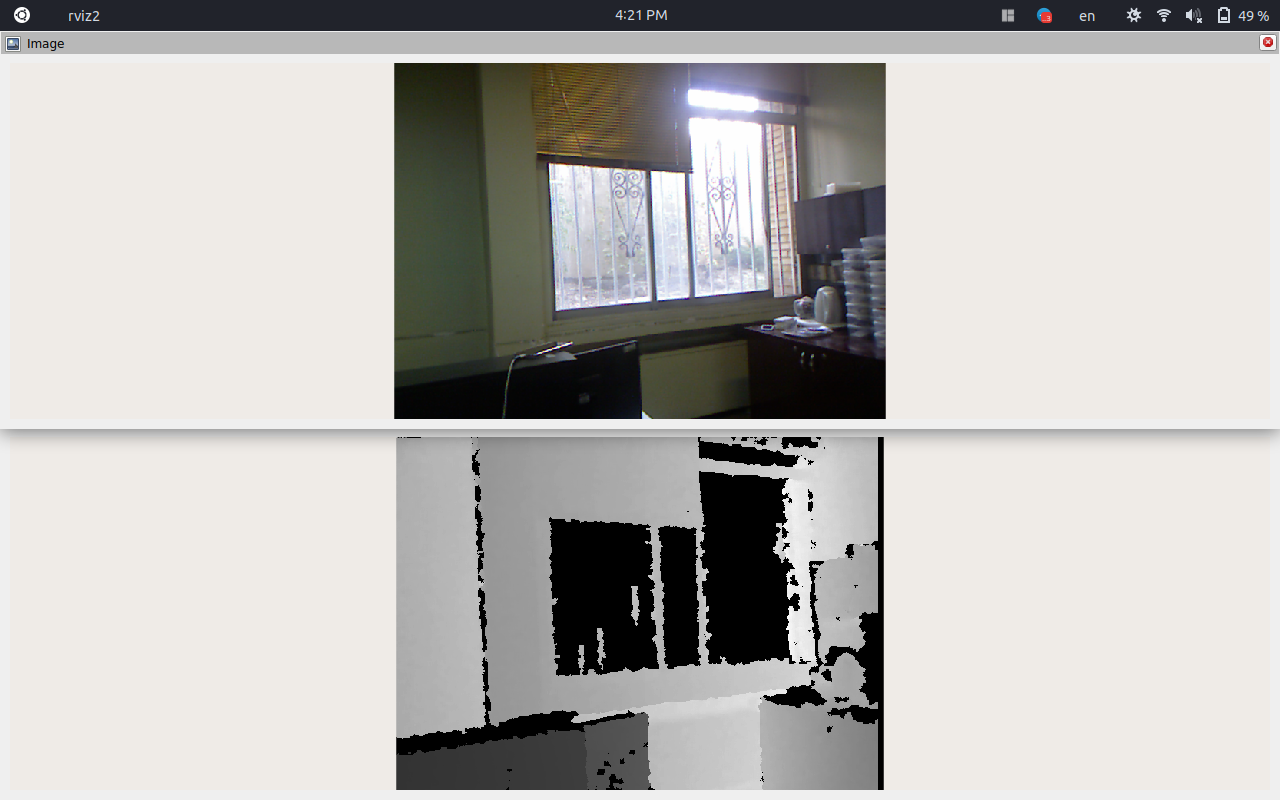
\includegraphics[width=0.8\linewidth]{figures/kinect-test.png}
	\caption{Testing kinect}
	\label{fig:kinectTest}
\end{figure}

One of the issues we encountered was the presence of out-of-sync timestamps between the \textcolor{ForestGreen}{\texttt{"camera\_info"}} and \textcolor{ForestGreen}{\texttt{"depth/camera\_info"}} topics that were being published. These two topics provide important calibration and intrinsic parameters for the RGB camera and the depth camera, respectively. Having these parameters synchronized correctly is crucial for accurate perception and 3D reconstruction.
When performing coordinate transformations between RGB and depth images or other perception tasks, using unsynchronized timestamps can lead to misalignments and inaccurate results. This affects the quality of visual data and hinders the performance of perception algorithms. Also in applications like mapping and navigation, incorrect timestamps can introduce errors in robot localization and obstacle avoidance. These errors can potentially lead to collisions or inefficient path planning. Accurate timestamps are crucial for correctly associating corresponding data from different sensors or perception modules. With out-of-sync timestamps, the associations can become incorrect, leading to flawed data interpretations.

To address this issue, we fixed the out-of-sync timestamps. We ensured that both topics publish their data with matching timestamps, ensuring that the calibration and intrinsic parameters correspond accurately to the corresponding RGB and depth images.
By resolving the timestamp synchronization problem, we improved the quality and reliability of our perception and mapping processes. It allowed our robot to better perceive and interpret the environment, leading to more accurate navigation and decision-making capabilities. As a result, the overall performance and robustness of our robot's perception system were greatly enhanced, allowing it to operate more effectively and efficiently in its environment.
%=========================================================================================================================
%-------------- 1.3 BRINGUP
%=========================================================================================================================
\subsection{Bringup}
After successfully setting up the Kinect package, we proceeded to bring up Eddie and test his movement. The steps we followed are as follows:
\begin{enumerate}
    \item Granting USB permissions: We connected the USB cable between Eddie and our laptop and executed the command "\textcolor{NavyBlue}{\texttt{sudo chmod a+rw /dev/ttyUSB0}}" to give the necessary permissions for communication with Eddie's control board.

    \item Bringing up Eddie: To initiate the robot's functionality, we ran the command "\textcolor{NavyBlue}{\texttt{ros2 launch eddiebot\_bringup eddie.launch.yaml}}" This command launched the required ROS2 nodes responsible for communicating with Eddie's control board and enabled communication within the ROS2 environment.

    \item Launching Navigation Stack: To enable navigation capabilities, we executed the command "\textcolor{NavyBlue}{\texttt{ros2 launch eddiebot\_nav eddiebot.launch.py}}" This step published static transforms specified in the eddiebot\_odom package and established transformations between the chassis and the base link of our sensors.

    \item Teleoperating Eddie: Finally, to control Eddie's movement, we ran the command "\textcolor{NavyBlue}{\texttt{ros2 run teleop\_twist\_keyboard teleop\_twist\_keyboard}}" This command allowed us to teleoperate Eddie by sending velocity commands to the robot, thus enabling movement in the desired direction.    
\end{enumerate}
By following these steps, we were able to successfully bring up Eddie, utilize the Kinect package for sensor data, and teleoperate the robot for movement using ROS2 commands. We could also bring up RViz to get a better sense of how Eddie is being represented in the ROS2 environment.

You can see our attempt at teleoperating Eddie \href{https://youtu.be/LtZwPk3DaKk}{here}.
%=========================================================================================================================
%-------------- 1.4 NETWORKING
%=========================================================================================================================
\subsection{Networking}
To enable teleoperation of Eddie using two laptops, we need to ensure that both laptops are connected to the same network. This allows them to communicate with each other. In ROS2, the default middleware for communication is DDS (Data Distribution Service). DDS utilizes the concept of Domain ID to enable different logical networks to share a physical network.

In ROS2, nodes within the same domain can discover and exchange messages with each other, while nodes in different domains cannot. By default, all ROS2 nodes use domain ID 0. The domain ID is used by DDS to calculate the UDP ports for discovery and communication. When a node starts, it broadcasts its presence to other nodes on the network within the same ROS domain, which is determined by the \textcolor{BrickRed}{\texttt{ROS\_DOMAIN\_ID}} environment variable. Nodes respond with their information, allowing the necessary connections to be established for communication between nodes.

By connecting the laptops in this manner, we can proceed with teleoperating Eddie. We can bring up rviz on the remote laptop, and configure it to display the RGB image from the Kinect sensor. This enables visualization of the camera feed on the remote laptop, providing a convenient way to monitor Eddie's environment during teleoperation.

